\documentclass[a4paper,12pt]{article}


\usepackage{natbib}

\usepackage{float}

\usepackage[utf8]{inputenc}

%Rajoute des régles de typo
\usepackage[french]{babel}
%Change l'accent
\usepackage[T1]{fontenc}
\usepackage{hyperref}
\usepackage{enumitem}
\usepackage{amsmath,amssymb}

\usepackage{color}

\usepackage{graphicx,xcolor}
\usepackage{geometry}
\geometry{left=1.5cm, right=1.5cm, bottom=2cm, }
\newcommand{\rmq}[1]{\textcolor{red}{#1}}

%Pour les définitions
\usepackage{amsthm}
\newtheorem{mydef}{Definition}

\begin{document}

	\newcommand{\HRule}{\rule{\linewidth}{0.5mm}}

	\begin{titlepage}

		\center

		\textsc{\LARGE Sorbonne université}\\[1.5cm] % Name of your university/college

        \begin{minipage}{0.4\textwidth}
		\begin{flushleft} \large
		\end{flushleft}
		\end{minipage}




		\textsc{\huge \bfseries Rapport de ARF}\\[.5cm]

		\HRule \\[0.4cm]
		{ \huge \bfseries TME 1 - 6 }\\[0.4cm]
		\HRule \\[4cm]

		{ \huge \textsc{Samu Tamminen} }

		\vfill
		Année 2017-2018
	\end{titlepage}



\newpage
\tableofcontents
\newpage

\section{TME 1 : Arbres de décision, sélection de modèles}

\subsection{Q1.3 Interpretation de l'entropie}
Calculer également la différence entre l’entropie et l’entropie conditionnelle pour chaque attribut.
A quoi correspond une valeur de 0 ? une valeur de 1 ? Quel est le meilleur attribut pour la première partition?
\\
Quand la différence entre l'entropie et l'entropie conditionnelle est 0 quand la partition n'est pas du tout bon et un,
quand la partition est le meilleur possible.

\subsection{Q1.4 - 6 La profondeur d'arbre }

En augmentant la profondeur maximale d'arbre, on obtient meilleur score.
Mais ces scores ne sont pas un indicateur fiable, si nous ne faisons pas différence entre les données training et test.

\subsection{Q1.7 -  Sur et sous apprentissage }

Le partition 0.8 / 0.2 dans figure ~\ref{fig:partition_8_2} semble d'etre le plus robust pour test et training.

Quand il y a que peu d'examples d'apprentissage, l'erreur est plus éleve dans le test.
Par contre quand on a beacoup des d'examples d'aprentissage, l'erreur dans le test est moins d'élevé.

\begin{figure}
\label{fig:partition_2_8}
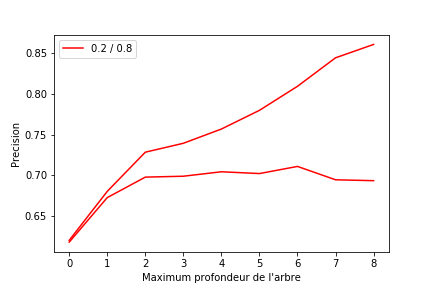
\includegraphics[width=0.4\linewidth]{images/tme1/partition_2_8.png}
\caption{Donnée aprentissage et test : 0.2 / 0.8}
\end{figure}

\begin{figure}
\label{fig:partition_5_5}
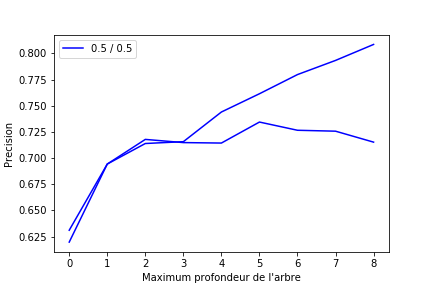
\includegraphics[width=0.4\linewidth]{images/tme1/partition_5_5.png}
\caption{Donnée aprentissage et test : 0.5 / 0.5}
\end{figure}

\begin{figure}
\label{fig:partition_8_2}
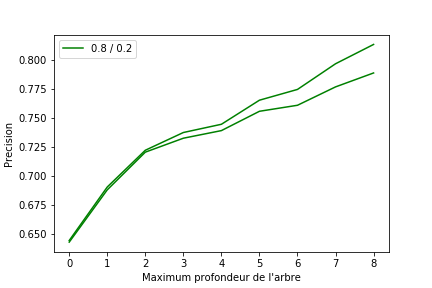
\includegraphics[width=0.4\linewidth]{images/tme1/partition_8_2.png}
\caption{Donnée aprentissage et test : 0.8 / 0.2}
\end{figure}

\section{TME 2 : Estimation de densité}

\section{TME 3 : Descente de gradient}

\section{TME 4 et 5 : Perceptron}

\section{TME 5 : Support Vector Machine}


\subsection{Pistes de recherche}

\end{document}
